The performance of ML algorithms is highly-dependent on the properties of the data. In the case of private learning, the constraints imposed by DP create additional challenges, and hence having fixed parameter settings is even less likely to perform well, leading to low accuracy or high privacy budget consumption (i.e., low protection). A significant amount of research explored the idea of adapting parameter values to the training data, or to other inputs such as number of iterations, batch size, privacy budget, learning rate, etc.~\cite{RefWorks:RefID:35-pichapati2019adaclip:,RefWorks:RefID:38-koskelalearning,RefWorks:RefID:48-fay2023adaptive}. %Typically, parameter values change at each step to fit the current iterations requirement. 

%Although we have only briefly discussed the idea of adaptive clipping in subsection 3.2.1, other parameters are also beings considered for adaptivity, including the learning rate and the privacy budget. 
In this section, we review several adaptive DP-SGD approaches, which fall mainly into three categories: tuning the privacy budget over time, varying the clipping threshold, or changing the learning rate. Adjusting these parameters offers several advantages. For instance, once can directly control the privacy budget consumption, which in DP-SGD is an output of the noise injection procedure (whereas the input is represented by noise magnitude). Furthermore, the privacy/accuracy trade-off of DP-SGD~\cite{RefWorks:RefID:47-yu2019differentially} can be better controlled, as hyperparameter values can significantly affect the performance of trained models~\cite{RefWorks:RefID:39-he2022exploring}. However, in the case of private learning, selecting optimal hyperparameter values is a lot more challenging than in non-private learning, due to the fact that any information used in tuning them has to be itself sanitized, potentially leading to additional privacy budget consumption. In contrast, with non-private learning, one can rely on trial-and-error approaches to do an exhaustive search of the hyperparameter space. Although some existing works have explored the problem or private hyperparameter tuning, they typically do not guarantee optimality of parameters, and they often increase the privacy budget consumed~\cite{RefWorks:RefID:52-liu2019private}.
 
\subsection{Privacy Budget Adaptation}
\label{secPri}
Perhaps the most challenging task in DP-SGD is striking a good trade-off between privacy and utility. DP-SGD injects noise into the gradient values during the training process to ensure that individual data points do not significantly influence the model updates in a way that allows re-identification. However, the noise addition process also degrades the quality of the learned model, leading to a reduction in its performance on the task at hand~\cite{RefWorks:RefID:40-abadi2016deep}. Hence, a delicate balance must be achieved between preserving the privacy of sensitive data and maintaining the effectiveness of the trained machine learning model. Next, we review three directions in which this trade-off can be controlled.



\subsubsection{Noise Decay}
\label{decay}

The first study that addressed adapting the DP-SGD privacy budget~\cite{RefWorks:RefID:47-yu2019differentially} proposed a solution based on the idea that, as the model converges, the gradient is expected to have a lower magnitude, thus allowing the learning process to converge faster to a local optimal, and achieve higher accuracy. To this end, a set of methods for privacy budget allocation were defined in~\cite{RefWorks:RefID:47-yu2019differentially} that dynamically reduce the noise scale as the training time increases. 
\begin{itemize}
    \item \textbf{Adaptive Schedule Based on Public Validation Dataset:} 
As mentioned earlier, one challenging aspect when making data-dependent decisions with private algorithms is that one must consume privacy budget when accessing any data-derived intermediate results. When public datasets are available, this challenge is averted, as one does not need to protect the inputs of the parameter tuning strategy algorithm. 

    The main idea in this approach is to continuously check the validation error on the {\em public} dataset while training on the private one, and dynamically reduce the noise scale whenever the validation accuracy improves by less than a set threshold $\delta$. In such cases, the noise scale is reduced by a factor of $k$ and this continues until the total privacy budget is consumed.
    %In their proposal, a public validation dataset is used to periodically assess the validation accuracy throughout the training process to ascertain whether the noise scale should be diminished for subsequent epochs. 
The evaluation intervals where validation is carried out are termed {\em validation epochs}.

Let $\sigma_e$ denote the noise scale for the DP-SGD training in validation epoch $e$, and $S_e$ represent the corresponding validation accuracy. The adjustment of the noise scale for subsequent epochs is contingent upon the discrepancy in accuracy between the current epoch $e$ and the preceding validation epoch $e - 1$. Initially, $S_0 = 0$.

The formula for adjusting the noise scale is:

\[
\sigma_e = \begin{cases} 
k \sigma_e, & \text{if } |S - S_{e-1}| \leq \delta \\
\sigma_e, & \text{otherwise} 
\end{cases}
\]

This adjustment ensures that the noise scale adapts based on the performance change observed between validation epochs. If the accuracy difference $S_e-S_{e-1}$ is less than the predetermined threshold $\delta$, the noise scale is attenuated by a factor of $k$ ($0<k<1$). To improve training effectiveness, the moving average of the validation accuracy is considered in the decision process, as there are cases where the validation accuracy does not increase monotonically within the training progress, and any fluctuations may result in unnecessary reduction of noise scale, which in turn consumes privacy budget.

    \item \textbf{Pre-defined Schedules: }
    In cases where a public validation dataset is not available, an alternative solution proposed in~\cite{RefWorks:RefID:47-yu2019differentially} calculates a fixed, data-independent schedule according to which the noise scale decreases over time. Four such decay strategies are presented:

\begin{enumerate}
    \renewcommand{\labelenumi}{\alph{enumi})}
    \item {\em Time-Based Decay}: the noise scale is adjusted using the formula $\sigma_t=\sigma_0/(1+kt)$, where $\sigma_0$ is the initial noise scale, $t$ is the number of training epochs so far, and $k>0$ is the decay rate. When $k<1$, this method is referred to as ``search-then-converge'', and the noise scale decreases linearly during the search phase when $t$ is less than the ``search time'' $1/k$; afterwards, the noise scale decreases by a factor of $1/t$.
    \item {\em Exponential Decay}: The noise scale decreases exponentially with each epoch, according to the expression $\sigma_t=\sigma_0e^{-kt}$, where $k>0$ is the decay rate.
    \item {\em Step Decay}: The noise scale decreases by an exponentially-increasing factor every few epochs, according to expression $\sigma_t=\sigma_0*k^{t/period}$. The decay rate $k$ is chosen such that $0<k<1$.
    \item {\em Polynomial Decay}: The noise parameter follows a polynomial decay function over a specified number of epochs $period$. Specifically,  $\sigma_t=(\sigma_0-\sigma_{end})*(1-t/period)^k+\sigma_\text{end}$ where $k>0$ is the decay rate and $t<period$. When $k=1$, this is referred to as a linear decay function.
\end{enumerate}

\end{itemize}
\subsubsection{Optimal Step Size Search}
\label{sec:step}
The previous approaches looked solely at how to adapt the privacy budget allocation throughout the learning process using different decay functions over time. Next, we look at an approach~\cite{concentrated} that adapts both the privacy budget and the learning rate (while we dedicate a separate section to learning rate adaptation approaches in Section~\ref{sec:lr}, we discuss this hybrid method here).
%The work in~\cite{concentrated} looks at how to find the optimal step based on a given set . B
At the core of the proposed technique from~\cite{concentrated} sits a privacy-preserving algorithm for computing the noisy maximum among the values in a set. The {\em NoisyMax} algorithm   adds independent Laplace noise to each set value and returns the index of the largest one, thereby providing differential privacy guarantees~\cite{concentrated}.

The two main components of the algorithms are {\em step-size selection} and {\em adaptive noise reduction}. The goal of step-size selection is to efficiently choose the per-iteration privacy budget. Adding noise to the gradients may not guarantee the correct direction of the descent, in expectation. To alleviate this issue, a portion of the privacy budget $p_\text{nmax}$ is used to check whether a given noisy estimate $\Tilde{g}_t$ of the gradient gives the correct descent direction. To accomplish this, a set $\Omega=\{f(w_t-\alpha\Tilde{g}_t):\alpha\in\Phi\}$ is constructed, where each element of the set is the objective value evaluated at $f(w_t-\alpha\Tilde{g}_t)$ and $\Phi$ is a set of pre-defined step-sizes. Using the NoisyMax computation, the algorithm calculates which step-size results in the smallest objective function value. Since an a priori bound cannot be determined on a given loss function $l$, gradient clipping is applied to bound sensitivity. This way, the first element of $\phi$ is fixed to $0$, to take into consideration the current objective value. Let $i$ be the index returned by the NoisyMax algorithm. If $i>0$, the algorithm updates $w_t$ using the chosen step size $a_i$. However, if $i=0$, $-\Tilde{g}_t$, it is likely that is not the correct descent direction, and none of the given step sizes will lead to a decrease in the value of the objective function $f$. Hence, the adaptive noise reduction is applied.

A block diagram of the NoisyMax technique is illustrated in Figure~\ref{fig:noisymax}. When the NoisyMax algorithm determines that the current gradient direction is incorrect, the algorithm increases the privacy budget used in noisy gradient approximation by a factor of $1 + y$. Using the gradient averaging technique, a total privacy budget of $p_\text{ng} – p_\text{old}$ is consumed to measure the new gradient with increased accuracy.  The gradient averaging technique is a method that recycles gradient estimates that were not useful by using the difference between two related privacy budget values to measure a new gradient, which when combined with the old measured gradient can be used to measure the final noisy gradient estimate at a lower privacy budget. Once the algorithm measures a new gradient, it goes through the NoisyMax algorithm again to determine its direction. These steps repeat until a good descent direction can be found.

\begin{figure}[h]
\centering
    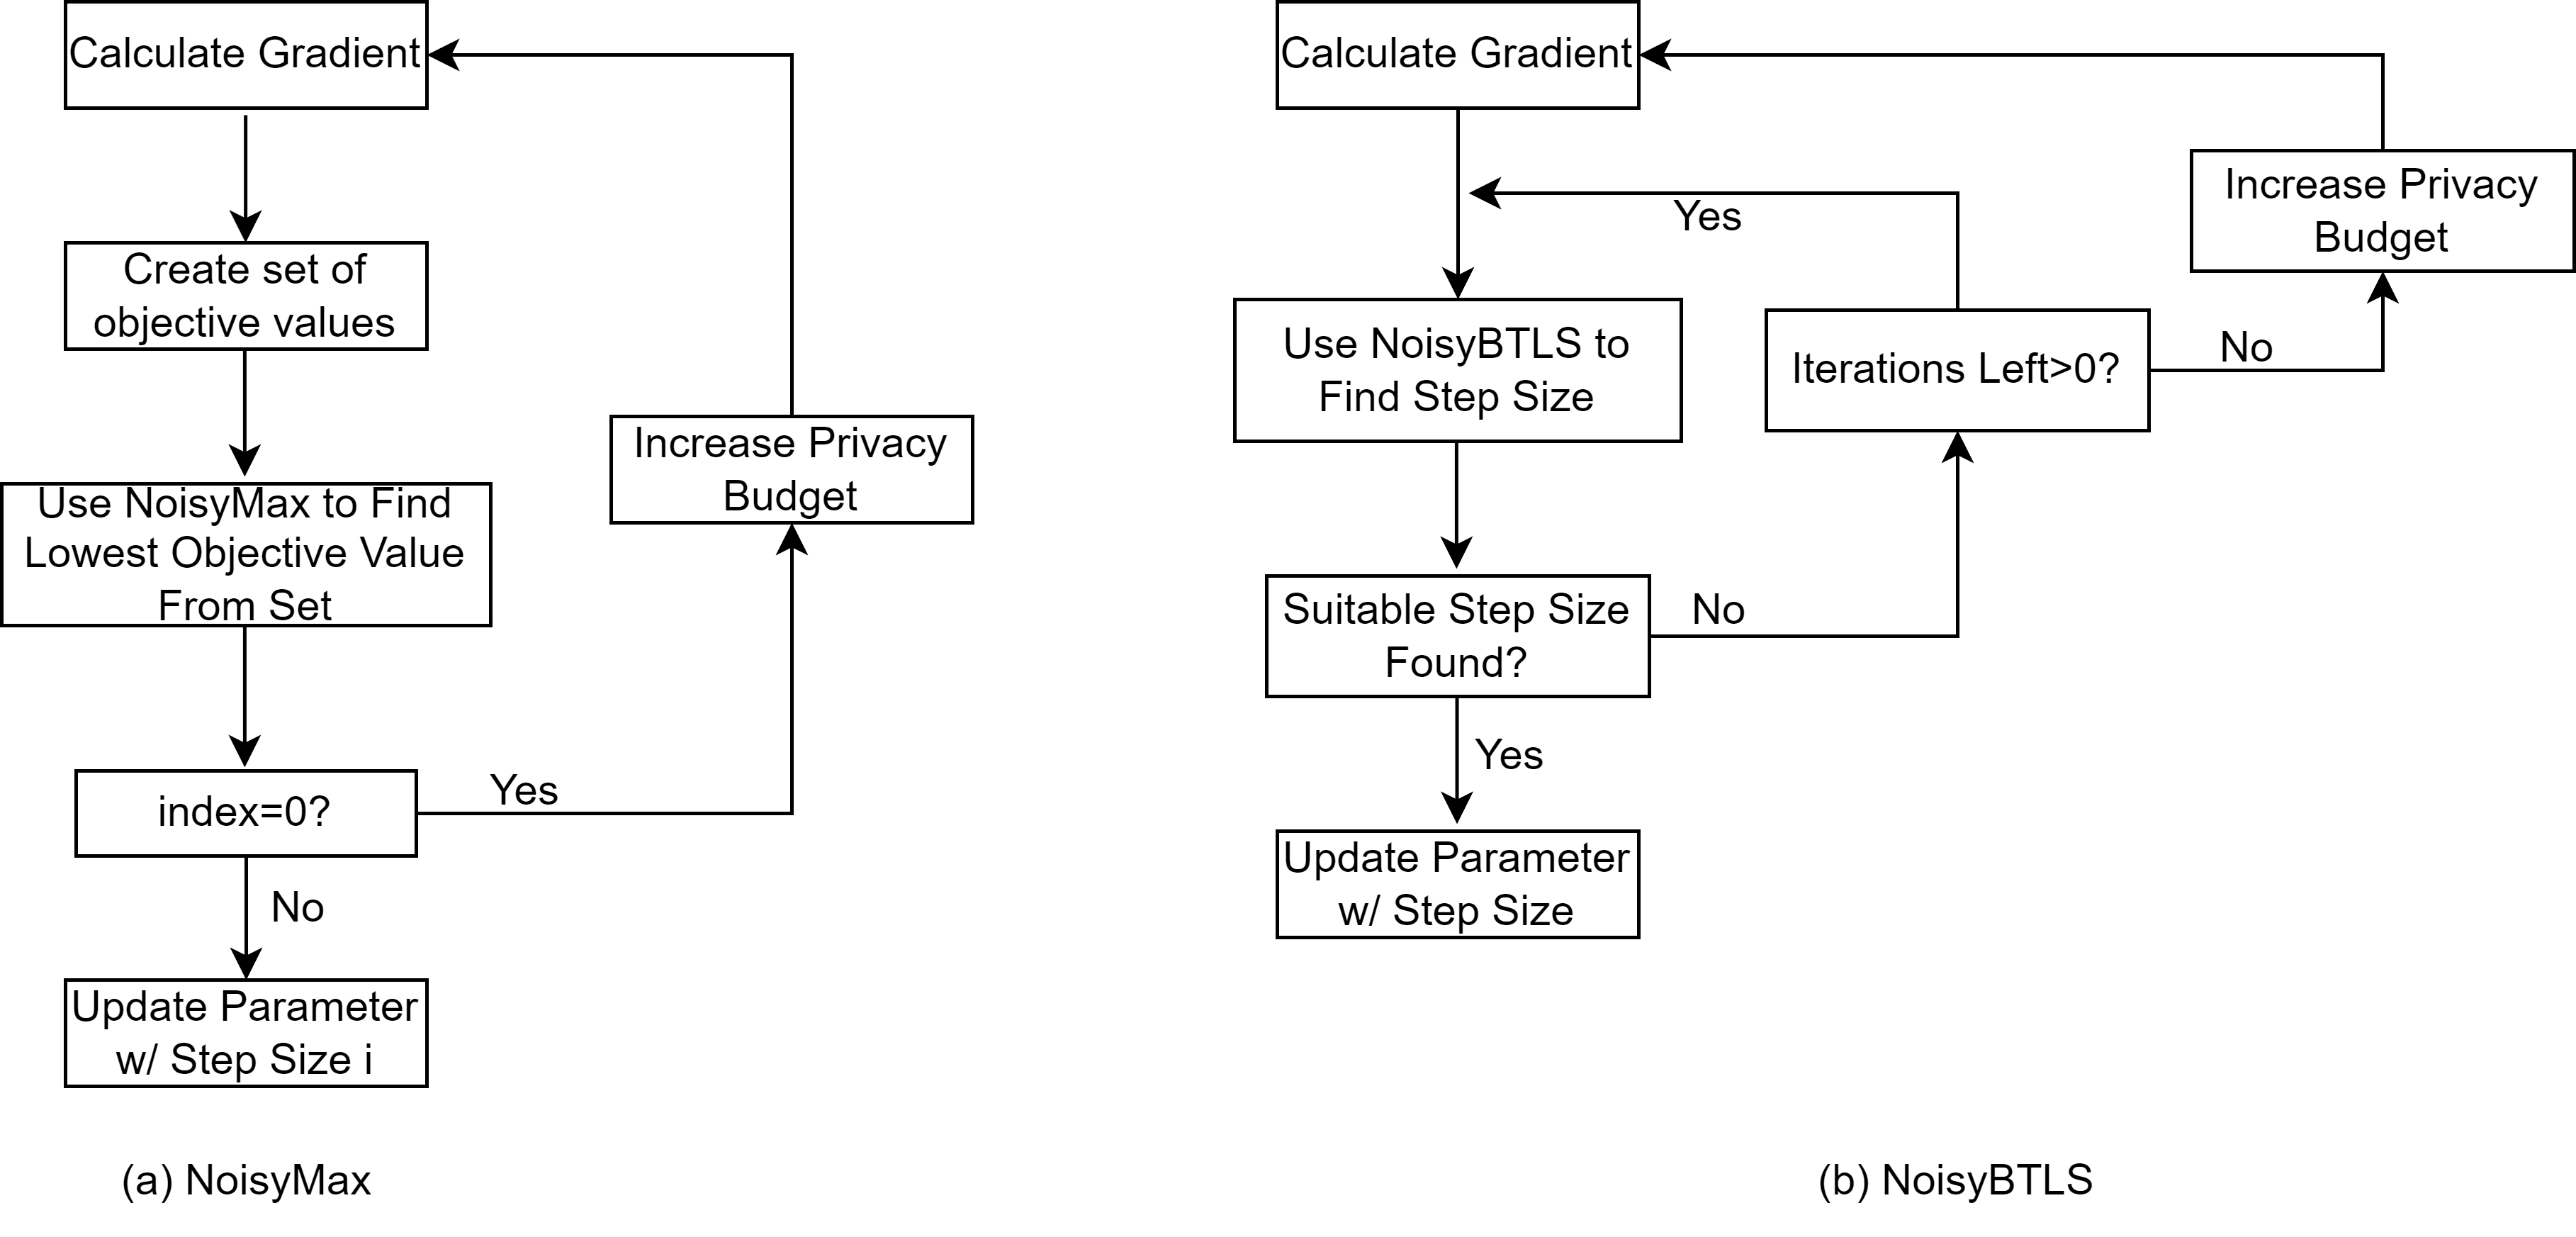
\includegraphics[width=1\linewidth]{submissions/submission5/figs/NoisyMax vs NoisyBTLS2.png}
   \caption{(a) NoisyMax Technique; (b) NoisyBTLS Technique}
   \label{fig:noisymax}
\end{figure} 

As an extension to NoisyMax, the same authors proposed a more advanced approach called Noisy Backtracking Line Search (NoisyBTLS). Similar to NoisyMax, NoisyBTLS adapts both the learning rate and the privacy budget, but in addition it also considers adaptive clipping (which is covered in more detail in Section~\ref{sec:adaclip}).

This method focuses on adapting the learning rate in response to noisy gradient computation while also adjusting the privacy budget using Sparse Vector Technique (also known as the ``above-threshold'' mechanism)~\cite{RefWorks:RefID:61-roth2011interactive,RefWorks:RefID:62-hardtmultiplicative}.
The approach first conducts a backtracking line search in a differentially private manner. %This algorithm is an implementation of the {\em above-threshold} mechanism~\cite{RefWorks:RefID:61-roth2011interactive,RefWorks:RefID:62-hardtmultiplicative}, also known as the {\em Sparse Vector Technique (SVT)}, for the task of line search. 
Figure~\ref{fig:noisymax}(b) illustrates this approach. The algorithm starts by introducing noise to the threshold \( T=0 \), resulting in a noisy threshold \( T=\lambda \), where \( \lambda \) is randomly drawn from a Laplace distribution or alternatively, a Gaussian distribution. Next, multiple iterations are performed, and in each one the following queries are evaluated:

\[ q(\eta,D)=f(w)-f(w-\eta\nabla f(w))-\alpha\eta\|\nabla f(w)\|^2 \]

with added noise \( \nu \) at each iteration. The result is compared with the noisy threshold \( T \). If \( q(\eta,D)+\nu\geq T \), the algorithm outputs \( \eta \) and halts; otherwise, it reduces the step size \( \eta \) by multiplying it with \( \beta \) and continues to the next iteration, where \( \beta\in(0,1) \) controls the rate of step size reduction. This process repeats for a maximum number of iterations. If no limit is set, depending on the noise used in the query, the iteration could lead to an infinite loop or provide minuscule step sizes, which could end up increasing the objective function due to a lack of progress. When the maximum number of iterations is reached, it statistically calculates whether a higher privacy budget is needed, which it then adjusts depending on the results. Due to the use of SVT, the privacy budget needed to find $\eta$ is greatly reduced.

When NOISYBTLS fails to find a step size within the set maximum iteration count, it can lead to two possibilities. The first one is that the current privacy budget $p_{grad}$ is set too small, and the noise dominates the gradient -- Case (1) in the diagram. In this case, the privacy budget needs to be increased. The second possibility is that the noise used in NOISYBTLS is too large and it can’t identify a step size with the right conditions -- Case (2) in the diagram. The remedy to this problem is to increase the privacy budget in order to compute a more precise gradient. To identify which of these two cases are applicable,  the algorithm maintains the moving average of angles between two consecutive gradient values, which gets updated at every iteration:

\[ \theta \leftarrow \text{ANGLE BETWEEN}(g_{t},\tilde{g}_{t})\]
\[\theta = \psi\theta + (1 - \psi)\theta_{t-1} \]

where $\psi \in (0,1)$ is a parameter controlling the decay rate of old information. When $\eta=0$ is returned by NOISYBTLS, the algorithm calculates another gradient $\tilde{g}_{t2}$ using the budget of $\rho_{\text{grad}}$ and measures the angle $\theta$ between $\tilde{g}_t$ and $\tilde{g}_{t2}$). The value of $\theta_{t2}$ is then compared with the moving average-based threshold $\theta_\text{max}$, and if it is larger it would increase the privacy budget $\p_\text{grad}$ for calculating the gradient. Meanwhile, if $\theta$ is less than the minimum threshold $\theta_\text{min}$, the search might fail due to insufficient privacy budget $\epsilon_{BT}$ for the NOISYBTLS. The threshold values $\theta_{\text{max}}$ and $\theta_{\text{min}}$ are calculated as follows:
\[ \theta_{\text{max}} = \phi_{\text{max}} \times \theta, \quad \theta_{\text{min}} = \phi_{\text{min}} \times \theta \]
where $\phi_{\text{max}} > 1$ and $0 < \phi_{\text{min}} < 1$ are hyperparameters. Empirically, this budget adaptation strategy is observed to be particularly effective for convex optimization problems.

In addition to adjusting the privacy budget, it was found that a large clipping threshold is not necessary in the later stages of the training process. Knowing this, the clipping threshold $C_\text{grad}$ and $C_\text{obj}$ is adaptively decreased when the algorithm finds it needs to increase the privacy budget $p_\text{grad}$ during a single SGD update. Even if $p_\text{grad}$ is increased multiple times in a single SGD update, the clipping threshold will only be updated once per update. The clipping threshold is updated as follows:
\[ C_{\text{grad}} \leftarrow (1-\zeta)C_{\text{grad}}, \quad C_{\text{obj}} \leftarrow (1-\zeta)C_{\text{grad}} \]
where $\zeta$ is a hyperparameter that determines the rate of decrease. Since the condition is based on privately released information, it does not consume any extra privacy budget.

\subsubsection{Convergence Rate}
%Above mentioned adaptation trials focus on increasing the privacy budget whenever an optimal step-size cannot be determined. 
Another recent approach to adapting the privacy budget consumption relies on convergence rates~\cite{RefWorks:RefID:49-hong2022dynamic}.
To assess the effectiveness of Private Gradient Descent (PGD), this work utilizes the Expected Excess Risk (EER), a common metric for evaluating the convergence of randomized algorithms. Given the presence of noise and the constraint on learning iterations, optimization using private gradients is expected to lead to a higher loss (excess risk) compared to the optimal solution without privacy constraints. Let \( \theta^* \) be the optimal solution obtained after iterating an algorithm  for \( T \) times. EER quantifies the expected utility degradation as:

\[
\text{EER} = \mathbb{E}[f(\theta_{\nu}^{T+1})] - f(\theta^*).
\]

Due to the variety of loss functions and complexity of recursive iterations, a good estimation of EER in the presence of noise is intractable for most functions. Instead, one can study the worst-case scenario, i.e., the upper bound of EER, with the goal to minimize the upper bound. For consistency, we refer to the upper bound of EER divided by the initial error as \( ERUB \). Since the analytical form of EER is either intractable or complicated due to the recursive iterations of noise, studying \( ERUB \) is a convenient and tractable alternative. The upper bound often has convenient functional forms which are (1) sufficiently simple, so that they can be directly minimized, and (2) closely related to the landscape of the objective depending on both the training dataset and the loss function. As a consequence, it was used in previous literature for choosing hyperparameters. Denote by \( ERUB_{\text{min}} \) the achievable optimal upper bound by a specific choice of parameters, e.g., noise magnitude \( \sigma \) and \( T \).

One can define the influence of noise magnitude \( \sigma \) on EER as the derivative:

\[
q_t^* = \frac{\partial \text{EER}}{\partial \sigma_t}.
\]

Accordingly, one can approximate the EER shift as \( \Delta \sigma \) when \( \sigma \) increases by \( \Delta \sigma \). However, because the EER is strongly data-dependent, the derived \( q_t^* \) on a given dataset may not generalize to another dataset. Instead, one can consider a more general term based on \( ERUB \), i.e., \( q_t^* = \frac{\partial}{\partial ERUB} \sigma_t \).

The work in~\cite{RefWorks:RefID:49-hong2022dynamic} considers the class of loss functions satisfying the Polyak-Lojasiewicz (PL) condition, which bounds losses by their corresponding gradient norms. It is more general than the \( m \)-strongly convexity condition~\cite{RefWorks:RefID:63-polyak1963gradient}. If \( f \) is differentiable and \( M \)-smooth, then \( m \)-strongly convexity implies the PL condition.

The related method in~\cite{RefWorks:RefID:48-fay2023adaptive}  introduces a conceptual framework aimed at dynamically adjusting hyperparameters over time by optimizing the privacy-utility ratio (PUR) at each step. This involves selecting the step size $\eta$ and noise standard deviation $\sigma$ to minimize the privacy loss per unit of utility improvement. The PUR is defined as the ratio of the privacy cost to the utility gain, with utility incorporating convergence metrics like the gradient norm or objective value. Minimizing the PUR enables adaptation of the privacy budget based on optimization progress, with higher precision typically required in later stages as the gradient norm diminishes near the optimum.

Two selection strategies emerge:


\textbf{1. Data-dependent selection:}
   By assuming $F$ is $M$-smooth, a descent lemma estimates the expected improvement in the objective function given step-size and noise variance. Using this lower bound as utility function, along with the privacy cost, one determines hyperparameters that minimize the privacy-utility ratio. Specifically, the privacy-utility ratio is minimized by setting the noise standard deviation $\sigma_t$ proportional to the gradient norm and the step size $\eta_t$ as a constant, given by:
   
   \[ \sigma_t = \frac{\| \nabla F(\theta_t) \|}{\sqrt{d}} \]
   \[ \eta_t = \frac{1}{2M} \]


\textbf{2. Data-independent selection:}  
   A data-independent schedule can be derived based on the PUR-optimal schedule, which is proportional to the gradient norm. This schedule exhibits similar convergence rates to non-private gradient descent (GD), leveraging upper bounds on gradient norms as a proxy for the gradient norm itself.
   
\subsection{Gradient Clipping Adaptation}
\label{sec:adaclip}

The clipping threshold parameter is used to bound the sensitivity of each gradient. A low clipping parameter can result in information being destroyed, and may change the direction of the gradient step. Meanwhile, a high clipping bound increases the sensitivity of training and requires more noise to be added~\cite{RefWorks:RefID:40-abadi2016deep}. It is difficult to achieve a good fixed clipping parameter setting without looking at the training data. Furthermore, weight layers and bias layers need completely different clipping values to be optimal. To tackle this issue, several approaches proposed their own implementation of adaptive clipping. 
%From section 3, we can see how adaptive clipping can provide improvements to the model utility compared to a fixed clipping threshold, and 
In Section~\ref{sec:step} we briefly discussed one method that pairs adaptive clipping with other adaptive parameters. One important aspect is that in a private setup, using gradient norms for tuning requires them to be sanitized first, which means that a portion of the privacy budget must be allocated in each step to protect the norms~\cite{RefWorks:RefID:39-he2022exploring}.

\subsubsection{Norm-based Adaptive Clipping}
\label{sec:normclip}
One of the first proposals of adaptive clipping was introduced by Van der Veen et.al.~\cite{RefWorks:RefID:36-lennarttools} who recognized that choosing a good clipping threshold $C$ is difficult, especially when dealing with multiple layers. They proposed that the clipping bound in the current batch be directly proportional to the $l_2$-norm of the previous batch by a constant factor $\alpha$. This can be summarized in the equation below: 

\[ C_t^l = \alpha|L|^{-1}(\sum_{i\in L_t}\text{clip}(||g_{t-1}^l(x_i)||_2)+\mathcal{N}(0,\sigma_{l^2}^2 C_{l^2t}^l ^2)\]
\[ \text{clip}(||y||_2)=||y||_2/\text{max}(1,\frac{||y||_2}{C_{l^2t}^l})\]

where $C_t^l$ is the clipping bound of the current round $t$ and layer $l$, $g_{t-1}^l(x_i)$  equates to the individual gradient of that layer in previous rounds and privacy parameters $\sigma_{l_2}$ and ${C_{l^2t}^l}$. To calculate the privacy parameter ${C_{l^2t}^l}$, an adaptive procedure is performed similar to clipping, where they sanitize the $l_2$-norm of the previous iteration, $C_{t-1}^l$, multiplied by a constant $\beta$, hence ${C_{l^2t}^l}=\beta C_{t-1}^l$. In this approach, it is required for the user to manually set the values of $\alpha$, $\beta$, and $\sigma_{l2}$, although it has been shown that changing the values of $\beta$ and $\sigma_{l2}$ does not provide meaningful results when measuring test accuracy. 
%Meanwhile, since the approach is adaptive, it is believed a single value of $\alpha$ can provide good results for all tasks.

\subsubsection{Quantile Estimation Adaptive Clipping}
\label{sec:quantile}
The recent work of He et.~al.~\cite{RefWorks:RefID:39-he2022exploring} explores an adaptive clipping technique that uses a form of quantile estimation in the context of per-layer clipping. A portion of the total privacy budget ($r=1\%$ to 10\% of total budget) is allocated for estimating the target quantile for each layer’s gradient norms. The clipping threshold for each layer $C_1,...,C_K$ is then set to the estimated quantile. The number of gradients clipped in each layer is recorded before each parameter update, and the clipping threshold is then adjusted based on how many individual gradients have been clipped previously. The fraction of clipped gradients needs to be sanitized according to DP, and an additional noise multiplier is used to achieve this goal. This also affects the noise multiplier setting for parameter updates, and the new noise multiplier is calculated as:
\[ \sigma_\text{new}=(\sigma^{-2}-K(2\sigma_b)^2)^{-1/2}\]
where $\sigma_b$ is the additional noise multiplier for the sanitized clipped gradients fraction, $\sigma$ is the original noise multiplier and $K$ is the number of layers in the neural network (also known as number of groups).

%The original Gaussian mechanism adds noise right before the release, meaning different coordinates uses the same amount of noise. However, 
The technique also uses different levels of noise in each layer. For example, let $\gamma_1,...,\gamma_k$ be coefficients for scaling, and $\Tilde{g}_k$ be the sum of clipped gradients for layer/group $k$. Applying the Gaussian mechanism to scaled $\hat{g}:= (\hat{g}_1,...,\hat{g}_k)$, where $\hat{g}_k:=\Tilde{g}_k/\gamma_k$, and rescaling back the sanitized values afterwards adds noise to $\Tilde{g}_k$ with standard deviation proportional to $\gamma_k$. There are two ways to choose $(\gamma_1,...,\gamma_K$):
\begin{itemize}
\item Global strategy: $\gamma_k=1$ for $k \in [K]$. This strategy adds same amount of noise to all components.
\item Equal budget strategy: $\gamma_k = C_k$ for $k \in [K]$. This strategy gives all the groups the same privacy budget.
\end{itemize}


Another method of adaptive gradient clipping has been explored in~\cite{RefWorks:RefID:37-andrewdifferentially}, this time in the context of federated learning (FL). %The main contribution to their approach is that proposed method uses negligible amount of privacy budget, and is also compatible with other FL technologies such as compression and secure aggregation. 
The main idea of the approach is to fix the quantile value of observed norms, and use gradient descent to fit $C$ to this value:
\[ \text{Let $X \in \mathbb{R}$ be a random variable, and let $\gamma \in [0,1]$ be a quantile to be matched. For any $C$, define}\] 
\[ l_\gamma (C,X)= 
\begin{cases}
    (1-\gamma)(C-X),& \text{if } X\leq C\\
    \gamma(X-C),              & \text{otherwise}
\end{cases}\]
which implies
\[
\nabla l'_y(C,X)=
\begin{cases}
    (1-\gamma)(C-X),& \text{if } X\leq C\\
    -\gamma,              & \text{otherwise}
\end{cases}
\] 
Since the loss is minimum when $Pr(X<C)=\gamma$, the loss function is convex and gradients are bounded by $1$, it is possible to get an online estimate of $C$ that converges to the $\gamma^\text{th}$ quantile of $X$ using online gradient descent. On a sample size $m$, with $b$ being the proportions of elements lower than $C$, the average derivative of the loss for that round can be simplified to $\Bar{b}-\gamma$. This is captured by the following equation:
\[ \Bar{l'}_\gamma (C;X)= \frac{1}{m}\sum_{i-1}^m
\begin{cases}
    (1-\gamma),& \text{if } x_i\leq C\\
    -\gamma,              & \text{otherwise}
\end{cases}\]
\[ =\frac{1}{m}((1-\gamma)\sum_{i\in [m]} \mathbf{I}_{x_i}\leq c-\gamma \sum_{i\in [m]} \mathbf{I}_{x_i}>c)=\Bar{b}-\gamma\] 
For a particular learning rate $\eta c$, the clipping bound can be updated through: $C\leftarrow C-\eta c(\Bar{b}-\gamma)$. Since $b$ and $\gamma$ take values in [0,1] the update clipping bound changes by at most $\eta \times c$ in each step. This can be a problem in two scenarios, one if $C$ is very large, and the other when updates are coarse and may overshoot to become negative if $C$ is a lot smaller than $\eta c$. The following geometric update rule can be used in this case: $C\leftarrow C \cdot \text{exp}(-\eta c(\Bar{b}-\gamma))$, which allows the update rule to quickly converge to the true quantile even if initial estimates are largely different. Figure ~\ref{AdaptiveClipping} illustrates the adaptive clipping algorithm using quantiles.

\begin{figure}[h]
\centering
    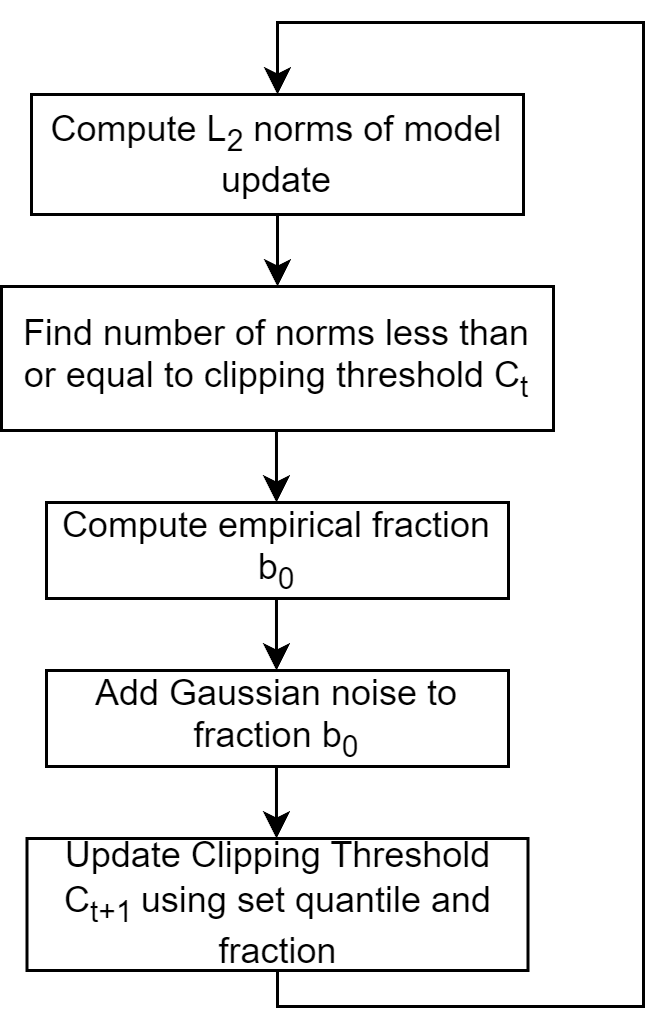
\includegraphics[width=0.3\linewidth]{submissions/submission5/figs/Quantile Estimation.png}
   \caption{Adaptive Clipping Using Quantiles}\label{FigDiff}
   \label{AdaptiveClipping}
\end{figure} 

\subsubsection{Coordinate-wise Adaptive Clipping}
The work of Pichapati et. al.\cite{RefWorks:RefID:35-pichapati2019adaclip:} proposed another approach to adaptive clipping. The {\em AdaClip} algorithm adds less noise compared to other methods by using {\em coordinate-wise} adaptive clipping of the gradient, as opposed to norm-based, thus producing models with improved accuracy. The main idea in the approach is rather than searching for a good clipping value, the gradients are centered and standardized before being clipped to $1$ and then noise is added to their value scaled according to the fixed sensitivity of $1$. The noisy values are then transformed back to their original mean and variance. 

Denote by $g^t$ the stochastic gradient vector at iteration $t$, and let $a^t$ and $b^t$ be auxiliary vectors. The gradient vector $g^t$ is first translated by $a^t$ obtaining $(g^t-a^t)$, then each dimension is divided by $b^t$. This produces the transformed gradient $w^t$, given by $w^t=\frac{g^t-a^t}{b^t}$. Sensitivity is bounded by clipping the transformed gradient at norm 1, according to equation:
\[ \hat{w}^t=\text{clip}(w^t,1)\overset{\Delta}{=}\frac{w^t}{\text{max}(1,||w^t||_2)}\]
Noise is then added to the clipped gradient:
\[ \Tilde{w}^t=\hat{w}^t+N^t\] \[ N^t\sim\mathcal{N}(0,\sigma^2I)\]
Finally, the noisy gradient is rescaled to the same scale as the original gradient by first multiplying with $b^t$ and then adding $a^t$:
\[ \hat{g}^t=b^t\hat{w}^t+a^t\]
This produces the differentially-private approximation of $g^t$. The main challenge consists in finding the optimal choices of the auxiliary vectors $a^t$ and $b^t$. When testing the implementation of AdaClip with the original DP-SGD implementation done by Abadi et al~\cite{RefWorks:RefID:40-abadi2016deep} on the MNIST dataset, AdaClip was found to produce higher accuracy for the same settings of $\varepsilon$ and $\delta$.


\subsection{Learning Rate Adaptation}
\label{sec:lr}
The learning rate parameter controls the step size taken during the optimization process to update the weights of the neural network. Choosing an optimal learning rate is very important: a small learning rate can result in the model taking too long converge, or being stuck at a local optimum. Meanwhile, a learning rate that is too large may result in a model that does not converge. %Typically, the choice of learning rate is done empirically through experimentation and validation, but the introduction of adaptivity allows the learning rate to be adjusted during the training process.

Adapting the learning rate is a concept that has been used in conventional, non-private machine learning, in tasks involving large-batch training~\cite{RefWorks:RefID:53-you2020large}.
%The main goal of adaptive learning rate is updating it depending on the level of trust in each update. Having more confidence in the gradient’s direction means that a larger learning rate can be set. 
In the context of DP-SGD, adapting the learning rate is even more important, as clipping and adding noise to gradients can change the direction of the gradient. %While we have explored solutions that adapted both the privacy budget and the learning rate at the same time in subsection 4.1.2, we will now look into a work that specifically targets learning rate adaptation.
\begin{figure}[h]
\centering
     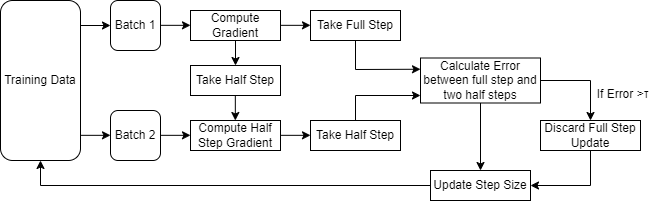
\includegraphics[width=1\linewidth]{submissions/submission5/figs/koskela.png}
   
   \caption{ADADP Update Mechanism}\label{FigDiff}
   \label{fig:koskela}
\end{figure} 

The most prominent approach using adaptive learning rate in private learning has been proposed in~\cite{RefWorks:RefID:38-koskelalearning} by Koskela et al. They proposed a method of adapting the learning rate by estimating the error against the gradient flow when comparing the results after one step and two half-steps. Figure~\ref{fig:koskela} provides an overview of how the algorithm functions, and how the step size is adaptively tuned. The basis of the approach relies on numerical extrapolation of ordinary differential equations (ODEs). Let $g$ be a differentiable function $g:R^d\rightarrow R$. To find the local minimum of function $g$, a first-order method called gradient descent (GD) is used. The gradient flow of $g$ can be described as the explicit Euler method with step size $\eta_l$ applied to a system of ODEs. An estimation of the error of the gradient descent can be performed by considering one step of size $\eta$:
\[ \theta_1=\theta_0-\eta \nabla g(\theta_0)\]
An alternative approach is to employ two steps of size $\frac{\eta}{2}$:
\[ \theta_{1/2}=\theta_0-\frac{\eta}{2}\nabla g(\theta_0) \qquad \hat{\theta}_1=\theta_{1/2}-\frac{\eta}{2}\nablag(\theta_{1/2})\]
It is thus possible to get an $O(\eta^3)$-accurate estimate of the local error through the value $2(\hat{\theta}_1-\theta_1)$. Using this information, the estimation of the error at iteration $l$ can be deduced from $\text{err}_l=||\hat{\theta}_{l+1}-\theta_{l+1}||$. The local error of magnitude $\tau$ to be desired is then set, which is used in the following proposed mechanism to update the step size:
\[ \eta_{l+1}=\text{min}(\text{max}(\frac{\tau}{\text{err}_l},\alpha_\text{min}),\alpha_\text{max})\cdot\eta_l \qquad \label{eq:koskela}\]
where the value of $\alpha_\text{min}<1$ and $\alpha_\text{max}>1$. 
%In the experiments done by this paper, the $\alpha_\text{min}<1$ was set to 0.9 while $\alpha_\text{max}>1$ was set to 1.1. 
When this mechanism is implemented in a DP-SGD setting, the equation to determine the local error is changed instead to be the estimate of the $\ell_2$-norm of the function $\text{err}(\theta,\hat{\theta})$ as it was found to give better numerical results.
\[ \text{err}(\theta,\hat{\theta})_i = \frac{|\theta_i-\hat{\theta}_i|}{\text{max}(1,|\theta_i|)}\]
The way the adaptive DP algorithm works is that a random batch $B_1$ is first drawn with probability $q=|B|/N$. The gradient $G_1$ is then calculated and clipped by $C$, before being evaluated at $\theta_l$. The algorithm then performs two different steps, one by step size $\eta_l$, $\eta_{l+1}\leftarrow\theta_l-\eta_lG_1$,  and the other by half step size, $\frac{\eta_l}{2}$, $\eta_{l+{1/2}}\leftarrow\theta_l-\frac{\eta_l}{2}G_1$. A second set of batches $B_2$ with probability $q$ is then drawn, gradient calculated and clipped $G_2$. This batch, however, is only being evaluated with the half-step size $\eta_{l+{1/2}}$ performed in the first batch, and another half step is performed, $\hat{\theta}_{l+1}\leftarrow\theta_{l+{1/2}}-\frac{\eta_l}{2}G_2$. The error between the updates done by one step size, $\theta_{l+1}$, and two half step size, $\hat{\theta}_{l+1}$ is then evaluated using $||\text{err}(\theta_{l+1}, \hat{\theta}_{l+1}||$. If the evaluated error is greater than the set tolerance parameter $\tau$, the updated parameter is discarded. Regardless of whether the updated parameter was kept or discarded, the next iteration step-size $\eta_$ is then calculated using equation~\eqref{eq:koskela}. 

One of the main advantages of this algorithm is that its privacy properties are simple to analyze. The complete algorithm can be modeled as $\Tilde{M}$ -- a composite of two different mechanisms: $M_{G_1}(X)$ and $M_{G_2}(X)$. The SGD approximation as well as the additive Gaussian noises are independent of each other, meanwhile, the sampling ratio $q$ is kept the same for both. By keeping parameters $q,\sigma$ and $C$ the same for both mechanism, the composite algorithm is able to run half as many iterations as DP-SGD to get the same privacy for the data.

One of the main difficulties in this implementation is choosing a good tolerance parameter $\tau$ that allows the accumulated additive noise to stay bounded as well as preventing any instabilities caused by the SGD gradient. This can be achieved by setting $\tau$ such that the accumulated DP noise after $T$ iterations is approximately $O(1)$ element-wise.

\subsection{Discussion}
\label{AdapDisc}
We explored several categories of techniques for adapting hyperparameters in DP-SGD, all targeting an improvement in the privacy-accuracy trade-off of learning. Table~\ref{tab: adapTable} provides a synthetic classification of the different methods covered in this section, and  the papers in which they were introduced. 
%Ultimately, the main goal of introducing adaptivity to DP-SGD is to improve the performance of the training process, thus increasing the overall accuracy of the model.
\begin{table}[]\centering
\caption{Summary Of Adaptive DP-SGD Approaches}\label{tab: adapTable}
\begin{tabular}{|c|ccc|}
\hline
\multirow{2}{*}{\textbf{Method}} & \multicolumn{3}{c|}{\textbf{Adaptive Hyperparameters}}                                                         \\ \cline{2-4} 
                                  & \multicolumn{1}{c|}{\textbf{Privacy Budget}} & \multicolumn{1}{c|}{\textbf{Clipping}} & \textbf{Learning Rate} \\ \hline
Noise Decay                       & \multicolumn{1}{c|}{\cite{RefWorks:RefID:47-yu2019differentially}}                        & \multicolumn{1}{c|}{}                  &                        \\ \hline
Optimal Step-Size Search          & \multicolumn{1}{c|}{\cite{concentrated},\cite{chen2020stochastic}}                        & \multicolumn{1}{c|}{}                  &    \cite{concentrated},\cite{chen2020stochastic}                    \\ \hline
Privacy-Based                     & \multicolumn{1}{c|}{}                        & \multicolumn{1}{c|}{\cite{chen2020stochastic}}                  &                        \\ \hline
Convergence Rate                  & \multicolumn{1}{c|}{\cite{RefWorks:RefID:49-hong2022dynamic},\cite{RefWorks:RefID:48-fay2023adaptive}}                        & \multicolumn{1}{c|}{}                  &                        \\ \hline
Norm-Based                        & \multicolumn{1}{c|}{}                        & \multicolumn{1}{c|}{\cite{RefWorks:RefID:36-lennarttools}}                  &                        \\ \hline
Quantile Estimation               & \multicolumn{1}{c|}{}                        & \multicolumn{1}{c|}{\cite{RefWorks:RefID:39-he2022exploring},\cite{RefWorks:RefID:37-andrewdifferentially}}                  &                        \\ \hline
Coordinate-wise                   & \multicolumn{1}{c|}{}                        & \multicolumn{1}{c|}{\cite{RefWorks:RefID:35-pichapati2019adaclip:}}                  &                        \\ \hline
Error Tolerance                   & \multicolumn{1}{c|}{}                        & \multicolumn{1}{c|}{}                  &     \cite{RefWorks:RefID:38-koskelalearning}                   \\ \hline
\end{tabular}
\end{table}

In the category of adapting the privacy budget, the advantage gained is achieved by fine-tuning the injected noise at different stages of learning. In the first few iterations, larger gradients are expected, hence a large privacy budget allocation may not help, but as the parameters approach their optimal values, gradients become smaller and require finer-grained tuning, hence the noise should be reduced~\cite{concentrated}. This aspect is further observed in the noise decay approaches, where a simple budget allocation strategy is able to achieve higher accuracy under fewer epochs compared to a uniform privacy budget~\cite{RefWorks:RefID:47-yu2019differentially}. However, that’s not to say the adaptive privacy budget is a perfect solution. There are usually constraints on where this approach is effective. For example, adapting the privacy budget based on the convergence rate requires making assumptions on the loss function, which is not always possible~\cite{RefWorks:RefID:48-fay2023adaptive}. Furthermore, some methods require a public validation dataset to be utilized, and when one is not available, the alternative approach requires setting some additional parameters, which can be difficult to optimize~\cite{RefWorks:RefID:47-yu2019differentially} and will consume budget otherwise allocated to computing gradients.
%This is not to mention the additional computational overhead required to monitor the gradient and make adjustments during each iteration. 

With adaptive clipping techniques, the main advantage gained is eliminating the need to fine-tune the clipping threshold parameter during training. We discussed earlier in the section the importance of setting a good clipping threshold, especially taking into account the sensitivity of the training process. Adaptive clipping helps balance the privacy-utility trade-off to a reasonable degree. In turn, this improves the stability of the training process, preventing extreme cases such as gradient explosions~\cite{RefWorks:RefID:37-andrewdifferentially}. In some cases, adaptive clipping is necessary to achieve good accuracy results compared to a fixed clipping threshold, as observed with per-layer clipping~\cite{RefWorks:RefID:39-he2022exploring}. It is also important to look at the drawbacks associated with adaptive clipping. Some methods, e.g., quantile estimation, require allocating some privacy budget to perform the necessary calculations~\cite{RefWorks:RefID:37-andrewdifferentially, RefWorks:RefID:39-he2022exploring}. Furthermore, a lot of the techniques used to implement adaptive clipping are dependent on additional hyperparameters in order to work, and depending on the sensitivity of these hyper-parameters the algorithm can influence the performance of adaptive clipping~\cite{RefWorks:RefID:35-pichapati2019adaclip:}. It is very difficult to choose an optimal value that can provide the best performance for each method.

The last adaptive hyperparameter we discussed is learning rate. The main advantage seen in adaptive learning rate is accelerating the convergence of the model during the training process. Dynamically adjusting the learning rate based on the gradient updates allows the model to make significant progress in a smaller number of iterations~\cite{RefWorks:RefID:38-koskelalearning}. This is especially the case during the early stages of training, when large model updates are beneficial as they accelerate convergence. However, it is important to factor in the additional computational overhead needed to adjust the learning rate at each iteration. This can end up causing the training time to significantly increase. Similarly to other adaptive techniques, some methods of adaptive learning rate are dependent on more hyperparameters that need to be carefully tuned for performance~\cite{RefWorks:RefID:38-koskelalearning}. It is also important to note that the performance of adaptive learning rate is highly dependent on the datasets and tasks being performed~\cite{concentrated}.

%Overall, introducing adaptive hyperparameters can be a great addition when looking for a boost in accuracy. It is important to consider which methods is most applicable to be used depending on the task that is being accomplished. One common drawback amongst all the adaptive hyperparameters is the need for additional hyperparameters. However, these papers often provides the optimal values needed to be set for each one. This may not be universally applicable depending on the dataset being worked on or the task being performed, but once these hyperparameters are tuned correctly an increase in accuracy and performance and sure to be gained.

